\documentclass[aspectratio=169]{beamer}
% Add slides directory to search path for Dartmouth theme
\makeatletter
\def\input@path{{../}}
\makeatother
\usetheme{Dartmouth}
\usepackage{graphicx}
\usepackage{tikz}
\usepackage{amsmath}
\usepackage{listings}
\usepackage{xcolor}
\usepackage{booktabs}
\usetikzlibrary{shapes,arrows,positioning,calc}

% Code listing setup
\lstset{
  basicstyle=\ttfamily\small,
  keywordstyle=\color{blue},
  commentstyle=\color{gray},
  stringstyle=\color{red},
  showstringspaces=false,
  breaklines=true,
  frame=single,
  language=Python
}

\title{Lecture 14: Training Transformers}
\subtitle{Week 5, Lecture 3 - From Architecture to Implementation}
\author{PSYC 51.07: Models of Language and Communication}
\date{Winter 2026}

\begin{document}

% ============================================================
% TITLE SLIDE
% ============================================================
\begin{frame}[shrink=10]
\titlepage
\end{frame}

% ============================================================
% OVERVIEW
% ============================================================
\begin{frame}[shrink=10]{Today's Agenda 📋}
\large
\begin{enumerate}\setlength{\itemsep}{0pt}
    \item 📍 \textbf{Positional Encoding}: Injecting sequence order
    \item 🔄 \textbf{Feed-Forward Networks}: The other key component
    \item 🔗 \textbf{Layer Norm \& Residuals}: Training deep networks
    \item ⚡ \textbf{FlashAttention}: Making transformers faster
    \item 🏗️ \textbf{Three Architectures}: Encoder, Decoder, Both
    \item 💻 \textbf{Practical Implementation}: Using HuggingFace
\end{enumerate}

\vspace{1em}
\textit{Goal: Complete understanding of transformer training and implementation}
\end{frame}

% ============================================================
% POSITIONAL ENCODING
% ============================================================
\begin{frame}[shrink=10]{Positional Encoding 📍}
\textbf{Problem: Self-attention is permutation-invariant!}

\vspace{0.5em}

Without position information:
\begin{itemize}\setlength{\itemsep}{0pt}
    \item "The cat sat" = "sat cat the" = "cat the sat"
    \item Order matters in language!
\end{itemize}

\vspace{1em}

\textbf{Solution: Add positional encodings to input embeddings}

\vspace{1em}

\begin{columns}[T]
\begin{column}{0.48\textwidth}
\textbf{Original Transformer (Sinusoidal):}
\begin{align*}
PE_{(pos, 2i)} &= \sin(pos / 10000^{2i/d}) \\
PE_{(pos, 2i+1)} &= \cos(pos / 10000^{2i/d})
\end{align*}

\textbf{Properties:}
\begin{itemize}\setlength{\itemsep}{0pt}
    \item Deterministic
    \item Unique for each position
    \item Smooth changes
    \item Generalizes to unseen lengths
\end{itemize}
\end{column}

\begin{column}{0.48\textwidth}
\textbf{Modern Approach: RoPE}

Rotary Position Embedding (Su et al. 2021)
\begin{itemize}\setlength{\itemsep}{0pt}
    \item Rotates Q and K in complex space
    \item Relative position encoding
    \item Better extrapolation
    \item Used in: LLaMA, GPT-NeoX
\end{itemize}

\vspace{1em}

\textbf{Learned Positional Embeddings:}
\begin{itemize}\setlength{\itemsep}{0pt}
    \item Treat positions as vocabulary
    \item Learn embeddings during training
    \item Used in: BERT, GPT
\end{itemize}
\end{column}
\end{columns}

\vspace{0.5em}
\small
\textit{References: Vaswani et al. (2017), Su et al. (2021) - "RoFormer: Enhanced Transformer with Rotary Position Embedding"}
\end{frame}

% ============================================================
% WHY SINUSOIDAL
% ============================================================
\begin{frame}[shrink=10]{Why Sinusoidal Positional Encoding? 🌊}
\textbf{Advantages of sine/cosine functions:}

\vspace{1em}

\begin{enumerate}\setlength{\itemsep}{0pt}
    \item \textbf{Unique Patterns}
    \begin{itemize}\setlength{\itemsep}{0pt}
        \item Each position gets a unique vector
        \item Different frequencies for different dimensions
        \item Creates distinguishable position signatures
    \end{itemize}

    \vspace{0.5em}

    \item \textbf{Relative Position Information}
    \begin{itemize}\setlength{\itemsep}{0pt}
        \item $PE_{pos+k}$ can be expressed as linear function of $PE_{pos}$
        \item Model can learn to attend by relative position
        \item Trigonometric identity: $\sin(a+b) = \sin a \cos b + \cos a \sin b$
    \end{itemize}

    \vspace{0.5em}

    \item \textbf{Extrapolation}
    \begin{itemize}\setlength{\itemsep}{0pt}
        \item Can handle sequences longer than training length
        \item Sine/cosine continue smoothly
        \item No need to retrain for different lengths
    \end{itemize}

    \vspace{0.5em}

    \item \textbf{No Additional Parameters}
    \begin{itemize}\setlength{\itemsep}{0pt}
        \item Deterministic, no learning required
        \item Saves memory compared to learned embeddings
    \end{itemize}
\end{enumerate}
\end{frame}

% ============================================================
% POSITIONAL ENCODING VISUALIZATION
% ============================================================
\begin{frame}[shrink=5]{Visualizing Positional Encodings 👁️}
\textbf{Each position gets a unique pattern across dimensions}

\vspace{1em}

\begin{center}
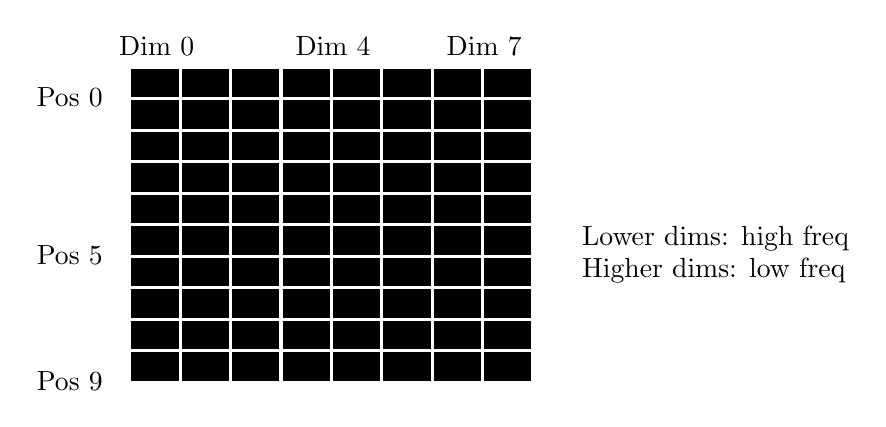
\begin{tikzpicture}[scale=0.8]
    % Draw a heatmap-like representation
    \foreach \pos in {0,...,9} {
        \foreach \dim in {0,...,7} {
            \pgfmathsetmacro{\val}{sin(\pos * 360 / (10000^(\dim/8)))}
            \pgfmathsetmacro{\color}{50 + 50*\val}
            \fill[blue!\color!red] (\dim*0.8, -\pos*0.5) rectangle ++(0.75, 0.45);
        }
    }

    % Labels
    \node[left] at (-0.3, 0) {Pos 0};
    \node[left] at (-0.3, -2.5) {Pos 5};
    \node[left] at (-0.3, -4.5) {Pos 9};

    \node[above] at (0.4, 0.5) {Dim 0};
    \node[above] at (3.2, 0.5) {Dim 4};
    \node[above] at (5.6, 0.5) {Dim 7};

    \node[right] at (7, -2.25) {Lower dims: high freq};
    \node[right] at (7, -2.75) {Higher dims: low freq};
\end{tikzpicture}
\end{center}

\vspace{0.5em}

\textbf{Key Insight:}
\begin{itemize}\setlength{\itemsep}{0pt}
    \item Lower dimensions: Rapid oscillation (high frequency)
    \item Higher dimensions: Slow oscillation (low frequency)
    \item Creates a unique "barcode" for each position
    \item Model learns to use these patterns for positional awareness
\end{itemize}
\end{frame}

% ============================================================
% FEED FORWARD
% ============================================================
\begin{frame}[shrink=5]{Feed-Forward Networks 🔄}
\textbf{After attention, apply position-wise feed-forward network}

\vspace{1em}

\textbf{Architecture:}
\begin{align*}
\text{FFN}(x) = \max(0, xW_1 + b_1)W_2 + b_2
\end{align*}

\begin{itemize}\setlength{\itemsep}{0pt}
    \item Two linear transformations with ReLU activation
    \item Applied to each position independently
    \item Same network for all positions
    \item Typical: Expand 4x then project back
\end{itemize}

\vspace{1em}

\begin{center}
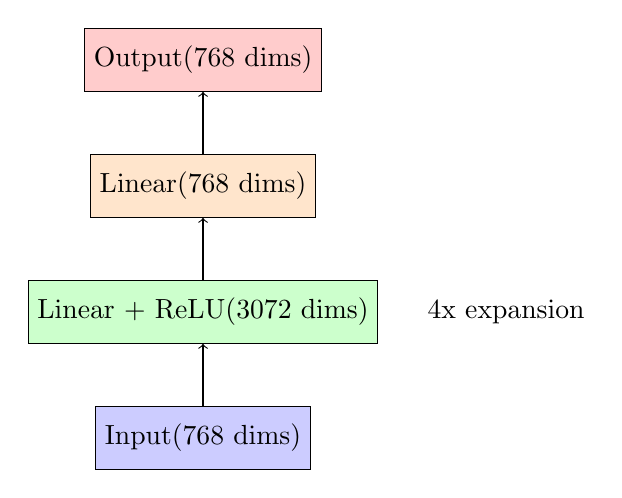
\begin{tikzpicture}[scale=0.8]
    \node[rectangle,draw,fill=blue!20,minimum width=2cm,minimum height=0.8cm] (input) at (0, 0) {Input\\(768 dims)};

    \node[rectangle,draw,fill=green!20,minimum width=2cm,minimum height=0.8cm] (expand) at (0, 2) {Linear + ReLU\\(3072 dims)};
    \draw[->] (input) -- (expand);

    \node[rectangle,draw,fill=orange!20,minimum width=2cm,minimum height=0.8cm] (project) at (0, 4) {Linear\\(768 dims)};
    \draw[->] (expand) -- (project);

    \node[rectangle,draw,fill=red!20,minimum width=2cm,minimum height=0.8cm] (output) at (0, 6) {Output\\(768 dims)};
    \draw[->] (project) -- (output);

    \node[right=0.5cm of expand] {4x expansion};
\end{tikzpicture}
\end{center}

\textbf{Purpose:} Add non-linearity and transform representations
\end{frame}

% ============================================================
% WHY FFN
% ============================================================
\begin{frame}[shrink=10]{Why Feed-Forward Networks? 🤔}
\textbf{Role in the Transformer:}

\vspace{1em}

\begin{enumerate}\setlength{\itemsep}{0pt}
    \item \textbf{Add Non-linearity}
    \begin{itemize}\setlength{\itemsep}{0pt}
        \item Attention is mostly linear operations (weighted sums)
        \item FFN introduces non-linear transformations
        \item ReLU/GELU activation adds expressiveness
    \end{itemize}

    \vspace{0.5em}

    \item \textbf{Position-wise Processing}
    \begin{itemize}\setlength{\itemsep}{0pt}
        \item Attention mixes information across positions
        \item FFN processes each position independently
        \item Allows position-specific feature transformations
    \end{itemize}

    \vspace{0.5em}

    \item \textbf{Increase Model Capacity}
    \begin{itemize}\setlength{\itemsep}{0pt}
        \item Expansion (4x) provides more parameters
        \item Can learn complex feature combinations
        \item Most parameters in transformer are in FFN layers!
    \end{itemize}

    \vspace{0.5em}

    \item \textbf{Feature Refinement}
    \begin{itemize}\setlength{\itemsep}{0pt}
        \item Attention gathers context
        \item FFN refines and transforms the representation
        \item Two complementary operations
    \end{itemize}
\end{enumerate}
\end{frame}

% ============================================================
% LAYER NORM AND RESIDUALS
% ============================================================
\begin{frame}[shrink=10]{Layer Normalization \& Residual Connections 🔗}
\textbf{Critical for training deep transformers!}

\vspace{1em}

\begin{columns}[T]
\begin{column}{0.48\textwidth}
\textbf{Residual Connections:}
\begin{align*}
\text{Output} = \text{Layer}(x) + x
\end{align*}

\begin{itemize}\setlength{\itemsep}{0pt}
    \item Allows gradients to flow directly
    \item Prevents vanishing gradients
    \item Enables very deep networks
    \item Identity mapping as fallback
\end{itemize}

\vspace{0.5em}

\textbf{Analogy:}
Like highway roads for information flow!
\end{column}

\begin{column}{0.48\textwidth}
\textbf{Layer Normalization:}
\begin{align*}
\text{LayerNorm}(x) = \gamma \frac{x - \mu}{\sigma} + \beta
\end{align*}

\begin{itemize}\setlength{\itemsep}{0pt}
    \item Normalize across features
    \item Stabilizes training
    \item Faster convergence
    \item Independent of batch size
\end{itemize}

\vspace{0.5em}

\begin{center}
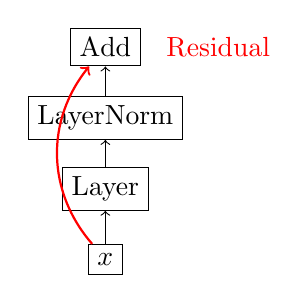
\begin{tikzpicture}[scale=0.6]
    \node[rectangle,draw] (x) at (0, 0) {$x$};
    \node[rectangle,draw] (layer) at (0, 1.5) {Layer};
    \node[rectangle,draw] (ln) at (0, 3) {LayerNorm};
    \node[rectangle,draw] (add) at (0, 4.5) {Add};

    \draw[->] (x) -- (layer);
    \draw[->] (layer) -- (ln);
    \draw[->] (ln) -- (add);
    \draw[->, thick, red] (x) to[bend left=40] (add);

    \node[red,right=0.2cm of add] {Residual};
\end{tikzpicture}
\end{center}
\end{column}
\end{columns}

\vspace{1em}

\textbf{Standard Pattern:}
\begin{align*}
x &\leftarrow \text{LayerNorm}(x + \text{MultiHeadAttention}(x)) \\
x &\leftarrow \text{LayerNorm}(x + \text{FFN}(x))
\end{align*}
\end{frame}

% ============================================================
% PRE VS POST NORM
% ============================================================
\begin{frame}[shrink=10]{Pre-Norm vs Post-Norm 🔄}
\small
\textbf{Two ways to arrange LayerNorm and residual connections}

\vspace{1em}

\begin{columns}[T]
\begin{column}{0.48\textwidth}
\textbf{Post-Norm (Original):}
\begin{align*}
x &\leftarrow \text{LN}(x + \text{Attn}(x)) \\
x &\leftarrow \text{LN}(x + \text{FFN}(x))
\end{align*}

\begin{itemize}\setlength{\itemsep}{0pt}
    \item Used in original Transformer
    \item Normalization after residual
    \item Better performance when it works
    \item \alert{Can be unstable for deep models}
    \item Requires careful initialization
\end{itemize}
\end{column}

\begin{column}{0.48\textwidth}
\textbf{Pre-Norm (Modern):}
\begin{align*}
x &\leftarrow x + \text{Attn}(\text{LN}(x)) \\
x &\leftarrow x + \text{FFN}(\text{LN}(x))
\end{align*}

\begin{itemize}\setlength{\itemsep}{0pt}
    \item Increasingly popular
    \item Normalization before sublayer
    \item \alert{More stable training}
    \item Easier to train very deep models
    \item Used in: GPT-2, GPT-3, many modern LLMs
\end{itemize}
\end{column}
\end{columns}

\vspace{1em}

\begin{block}{Recommendation}
For deep transformers (24+ layers), Pre-Norm is generally preferred due to better training stability.
\end{block}
\end{frame}

% ============================================================
% COMPLETE BLOCK
% ============================================================
\begin{frame}[shrink=5]{Complete Transformer Block 🧱}
\textbf{Putting it all together:}

\vspace{1em}

\begin{center}
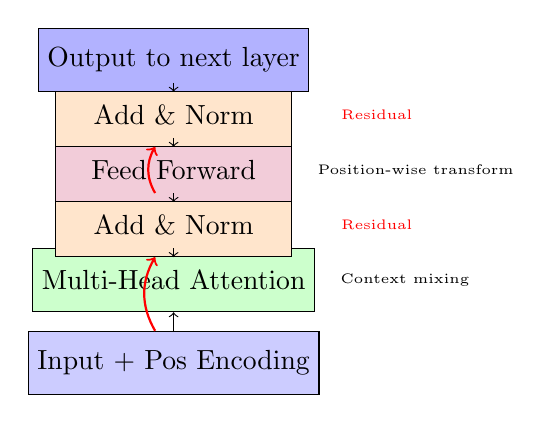
\begin{tikzpicture}[scale=0.7]
    % Input
    \node[rectangle,draw,fill=blue!20,minimum width=3cm,minimum height=0.8cm] (input) at (0, 0) {Input + Pos Encoding};

    % Multi-head attention
    \node[rectangle,draw,fill=green!20,minimum width=3cm,minimum height=0.8cm] (mha) at (0, 1.5) {Multi-Head Attention};
    \draw[->] (input) -- (mha);

    % Add & Norm 1
    \node[rectangle,draw,fill=orange!20,minimum width=3cm,minimum height=0.8cm] (an1) at (0, 2.5) {Add \& Norm};
    \draw[->] (mha) -- (an1);
    \draw[->, thick, red] (input) to[bend left=30] (an1);

    % Feed forward
    \node[rectangle,draw,fill=purple!20,minimum width=3cm,minimum height=0.8cm] (ffn) at (0, 3.5) {Feed Forward};
    \draw[->] (an1) -- (ffn);

    % Add & Norm 2
    \node[rectangle,draw,fill=orange!20,minimum width=3cm,minimum height=0.8cm] (an2) at (0, 4.5) {Add \& Norm};
    \draw[->] (ffn) -- (an2);
    \draw[->, thick, red] (an1) to[bend left=30] (an2);

    % Output
    \node[rectangle,draw,fill=blue!30,minimum width=3cm,minimum height=0.8cm] (output) at (0, 5.5) {Output to next layer};
    \draw[->] (an2) -- (output);

    % Labels
    \node[right=0.2cm of mha] {\tiny Context mixing};
    \node[right=0.2cm of ffn] {\tiny Position-wise transform};
    \node[right=0.5cm of an1, red] {\tiny Residual};
    \node[right=0.5cm of an2, red] {\tiny Residual};
\end{tikzpicture}
\end{center}

\vspace{0.5em}

\textbf{Stack this block $N$ times!}
\begin{itemize}\setlength{\itemsep}{0pt}
    \item BERT-base: 12 blocks
    \item BERT-large: 24 blocks
    \item GPT-3: 96 blocks!
\end{itemize}
\end{frame}

% ============================================================
% FLASH ATTENTION
% ============================================================
\begin{frame}[shrink=10]{FlashAttention: Making Transformers Faster ⚡}
\textbf{Problem: Standard attention is slow and memory-hungry!}

\vspace{0.5em}

\begin{alertblock}{Standard Attention Complexity}
\begin{itemize}\setlength{\itemsep}{0pt}
    \item Time: $O(n^2)$ where $n$ is sequence length
    \item Memory: $O(n^2)$ to store attention matrix
    \item Bottleneck: Reading/writing to GPU memory (HBM)
\end{itemize}
\end{alertblock}

\vspace{1em}

\begin{columns}[T]
\begin{column}{0.48\textwidth}
\textbf{FlashAttention Innovation:}
\begin{itemize}\setlength{\itemsep}{0pt}
    \item Tile-based computation
    \item Uses fast SRAM instead of slow HBM
    \item Fused operations
    \item Recomputation in backward pass
    \item \alert{2-4x faster!}
    \item Enables longer sequences
\end{itemize}
\end{column}

\begin{column}{0.48\textwidth}
\textbf{Impact:}
\begin{itemize}\setlength{\itemsep}{0pt}
    \item GPT-3: 512 → 2048 context
    \item BERT: Faster training
    \item Long-document understanding
    \item Used in: LLaMA, GPT-4
\end{itemize}

\vspace{1em}

\begin{center}
\begin{tabular}{lcc}
\toprule
\textbf{Method} & \textbf{Speed} & \textbf{Memory} \\
\midrule
Standard & 1x & 1x \\
FlashAttn & \textbf{3x} & \textbf{0.5x} \\
\bottomrule
\end{tabular}
\end{center}
\end{column}
\end{columns}

\vspace{0.5em}
\small
\textit{Reference: Dao et al. (2022) - "FlashAttention: Fast and Memory-Efficient Exact Attention"}
\end{frame}

% ============================================================
% OTHER OPTIMIZATIONS
% ============================================================
\begin{frame}[shrink=10]{Other Attention Optimizations ⚙️}
\textbf{Addressing the $O(n^2)$ problem:}

\vspace{1em}

\begin{enumerate}\setlength{\itemsep}{0pt}
    \item \textbf{Sparse Attention}
    \begin{itemize}\setlength{\itemsep}{0pt}
        \item Only attend to subset of positions
        \item Local windows + global tokens
        \item Used in: Longformer, BigBird
    \end{itemize}

    \vspace{0.5em}

    \item \textbf{Linear Attention}
    \begin{itemize}\setlength{\itemsep}{0pt}
        \item Approximate attention with linear complexity
        \item Kernel trick to avoid materializing attention matrix
        \item Used in: Performer, Linear Transformer
    \end{itemize}

    \vspace{0.5em}

    \item \textbf{Low-Rank Approximation}
    \begin{itemize}\setlength{\itemsep}{0pt}
        \item Factorize attention matrix
        \item Reduce memory footprint
        \item Used in: Linformer
    \end{itemize}

    \vspace{0.5em}

    \item \textbf{Sliding Window}
    \begin{itemize}\setlength{\itemsep}{0pt}
        \item Fixed-size local attention window
        \item Constant memory usage
        \item Used in: Mistral 7B
    \end{itemize}
\end{enumerate}

\vspace{0.5em}
\textbf{Trade-off:} Efficiency vs. expressiveness. Full attention often still best for quality.
\end{frame}

% ============================================================
% ENCODER VS DECODER VS BOTH
% ============================================================
\begin{frame}{Three Transformer Architectures 🏗️}
\begin{center}
\begin{tabular}{p{3cm}p{4cm}p{4cm}}
\toprule
\textbf{Architecture} & \textbf{How it works} & \textbf{Examples \& Uses} \\
\midrule
\textbf{Encoder-only} &
Bidirectional self-attention. Can see entire sequence. &
BERT, RoBERTa, ALBERT\\
\textit{Best for:} Classification, NER, QA \\
\midrule
\textbf{Decoder-only} &
Masked self-attention. Can only see past. Autoregressive. &
GPT, GPT-2, GPT-3, LLaMA\\
\textit{Best for:} Generation, completion \\
\midrule
\textbf{Encoder-Decoder} &
Encoder: bidirectional\\
Decoder: masked + cross-attention &
T5, BART, mT5\\
\textit{Best for:} Translation, summarization \\
\bottomrule
\end{tabular}
\end{center}

\vspace{1em}

\begin{block}{Key Difference: Attention Masking}
\begin{itemize}\setlength{\itemsep}{0pt}
    \item \textbf{Encoder:} Full self-attention (bidirectional)
    \item \textbf{Decoder:} Causal/masked attention (unidirectional)
\end{itemize}
\end{block}
\end{frame}

% ============================================================
% VISUAL ARCHITECTURES
% ============================================================
\begin{frame}[shrink=5]{Visual Comparison: Encoder vs Decoder vs Both}
\begin{center}
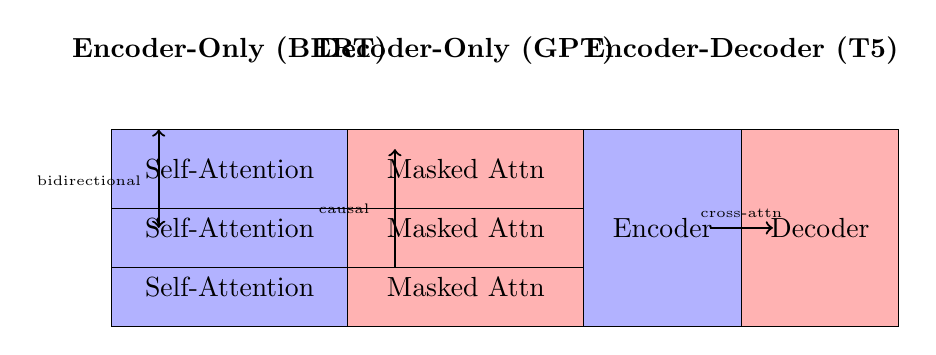
\begin{tikzpicture}[scale=0.5]
    % Encoder only (BERT)
    \node at (0, 6) {\textbf{Encoder-Only (BERT)}};
    \foreach \y in {0, 1.5, 3} {
        \node[rectangle,draw,fill=blue!30,minimum width=3cm,minimum height=1cm] at (0, \y) {Self-Attention};
    }
    \draw[<->, thick] (-1.8, 1.5) -- (-1.8, 4);
    \node[left] at (-2, 2.7) {\tiny bidirectional};

    % Decoder only (GPT)
    \node at (6, 6) {\textbf{Decoder-Only (GPT)}};
    \foreach \y in {0, 1.5, 3} {
        \node[rectangle,draw,fill=red!30,minimum width=3cm,minimum height=1cm] at (6, \y) {Masked Attn};
    }
    \draw[->, thick] (4.2, 0.5) -- (4.2, 3.5);
    \node[left] at (3.8, 2) {\tiny causal};

    % Encoder-Decoder (T5)
    \node at (13, 6) {\textbf{Encoder-Decoder (T5)}};
    \node[rectangle,draw,fill=blue!30,minimum width=2cm,minimum height=2.5cm] at (11, 1.5) {Encoder};
    \node[rectangle,draw,fill=red!30,minimum width=2cm,minimum height=2.5cm] at (15, 1.5) {Decoder};
    \draw[->, thick] (12.2, 1.5) -- (13.8, 1.5) node[midway,above] {\tiny cross-attn};
\end{tikzpicture}
\end{center}

\vspace{1em}

\textbf{Choosing the Right Architecture:}
\begin{itemize}\setlength{\itemsep}{0pt}
    \item Need to understand full context? → \textbf{Encoder} (BERT)
    \item Need to generate text? → \textbf{Decoder} (GPT)
    \item Need both (translate, summarize)? → \textbf{Encoder-Decoder} (T5)
\end{itemize}
\end{frame}

% ============================================================
% CODE EXAMPLE
% ============================================================
\begin{frame}[fragile]{Using Transformers in Practice 💻}
\textbf{HuggingFace makes it easy!}

\begin{lstlisting}[language=Python]
from transformers import AutoModel, AutoTokenizer

# Load pre-trained model
model_name = "bert-base-uncased"
tokenizer = AutoTokenizer.from_pretrained(model_name)
model = AutoModel.from_pretrained(model_name)

# Tokenize input
text = "The animal didn't cross the street because it was too tired"
inputs = tokenizer(text, return_tensors="pt")

# Get contextualized embeddings
outputs = model(**inputs)
hidden_states = outputs.last_hidden_state  # Shape: [batch, seq_len, 768]

# Extract embedding for specific token
token_embeddings = hidden_states[0]  # [seq_len, 768]
print(f"Shape: {token_embeddings.shape}")
# Each token now has a context-aware representation!
\end{lstlisting}

\vspace{0.5em}
\small
\textit{Reference: HuggingFace Course - Chapter 1.4 (How do Transformers work?)}
\end{frame}

% ============================================================
% DIFFERENT ARCHITECTURES CODE
% ============================================================
\begin{frame}[fragile]{Comparing Architectures: Code Examples 💻}
\textbf{Different architectures for different tasks}

\begin{lstlisting}[language=Python]
from transformers import AutoModelForSequenceClassification, \
                         AutoModelForCausalLM, \
                         AutoModelForSeq2SeqLM

# 1. ENCODER-ONLY (BERT): Classification
encoder_model = AutoModelForSequenceClassification.from_pretrained(
    "bert-base-uncased", num_labels=2
)
# Use for: Sentiment analysis, NER, classification

# 2. DECODER-ONLY (GPT): Text generation
decoder_model = AutoModelForCausalLM.from_pretrained("gpt2")
# Use for: Text completion, creative writing, few-shot learning

# 3. ENCODER-DECODER (T5): Seq2Seq tasks
seq2seq_model = AutoModelForSeq2SeqLM.from_pretrained("t5-base")
# Use for: Translation, summarization, question answering

# All use transformer architecture, different attention patterns!
\end{lstlisting}

\vspace{0.5em}
\textbf{Key Takeaway:} Choose architecture based on your task!
\end{frame}

% ============================================================
% TRAINING TIPS
% ============================================================
\begin{frame}[shrink=10]{Practical Tips for Training Transformers 💡}
\begin{enumerate}\setlength{\itemsep}{0pt}
    \item \textbf{Learning Rate \& Warmup}
    \begin{itemize}\setlength{\itemsep}{0pt}
        \item Use learning rate warmup (linear increase then decay)
        \item Typical: warmup for 10\% of training steps
        \item Peak LR: 1e-4 to 5e-4 (from scratch), 1e-5 to 5e-5 (fine-tuning)
    \end{itemize}

    \vspace{0.5em}

    \item \textbf{Optimization}
    \begin{itemize}\setlength{\itemsep}{0pt}
        \item Use Adam or AdamW optimizer
        \item AdamW: Adam + weight decay (better generalization)
        \item Gradient clipping to prevent exploding gradients
    \end{itemize}

    \vspace{0.5em}

    \item \textbf{Regularization}
    \begin{itemize}\setlength{\itemsep}{0pt}
        \item Dropout after attention and FFN (typical: 0.1)
        \item Weight decay (typical: 0.01)
        \item Label smoothing for classification
    \end{itemize}

    \vspace{0.5em}

    \item \textbf{Mixed Precision Training}
    \begin{itemize}\setlength{\itemsep}{0pt}
        \item Use FP16 instead of FP32
        \item 2x speedup, 2x memory reduction
        \item Minimal accuracy loss
    \end{itemize}
\end{enumerate}
\end{frame}

% ============================================================
% EFFICIENCY TIPS
% ============================================================
\begin{frame}[shrink=10]{Computational Efficiency Tips ⚙️}
\begin{enumerate}\setlength{\itemsep}{0pt}
    \item \textbf{Batch Size}
    \begin{itemize}\setlength{\itemsep}{0pt}
        \item Larger batches = better GPU utilization
        \item Use gradient accumulation if GPU memory limited
        \item Typical: effective batch size 256-2048 tokens
    \end{itemize}

    \vspace{0.5em}

    \item \textbf{Sequence Length}
    \begin{itemize}\setlength{\itemsep}{0pt}
        \item Shorter sequences train faster (quadratic complexity!)
        \item Consider truncation or sliding windows
        \item Pack multiple examples to maximize GPU usage
    \end{itemize}

    \vspace{0.5em}

    \item \textbf{Model Size}
    \begin{itemize}\setlength{\itemsep}{0pt}
        \item Start small, scale up if needed
        \item DistilBERT: 40\% smaller, 60\% faster, 97\% performance
        \item Consider model distillation for deployment
    \end{itemize}

    \vspace{0.5em}

    \item \textbf{Hardware}
    \begin{itemize}\setlength{\itemsep}{0pt}
        \item GPUs with high memory bandwidth (A100, H100)
        \item Multi-GPU training with data parallelism
        \item Use FlashAttention when available
    \end{itemize}
\end{enumerate}
\end{frame}

% ============================================================
% DISCUSSION
% ============================================================
\begin{frame}[shrink=10]{Discussion Questions 💭}
\begin{enumerate}\setlength{\itemsep}{0pt}
    \item \textbf{Positional Encoding:}
    \begin{itemize}\setlength{\itemsep}{0pt}
        \item Why add instead of concatenate?
        \item What happens without positional encoding?
        \item Learned vs. fixed: which is better?
    \end{itemize}

    \vspace{0.5em}

    \item \textbf{Architecture Choice:}
    \begin{itemize}\setlength{\itemsep}{0pt}
        \item When would you use encoder-only vs decoder-only?
        \item Can GPT do classification? Can BERT generate?
        \item Why has decoder-only become more popular recently?
    \end{itemize}

    \vspace{0.5em}

    \item \textbf{Scaling:}
    \begin{itemize}\setlength{\itemsep}{0pt}
        \item Is bigger always better?
        \item What are the limits to scaling transformers?
        \item How do we make them more efficient?
    \end{itemize}

    \vspace{0.5em}

    \item \textbf{Training Stability:}
    \begin{itemize}\setlength{\itemsep}{0pt}
        \item Why are residual connections so important?
        \item Pre-norm vs post-norm: trade-offs?
    \end{itemize}
\end{enumerate}
\end{frame}

% ============================================================
% LOOKING AHEAD
% ============================================================
\begin{frame}[shrink=10]{Looking Ahead to Week 6 🔮}
\textbf{This week (Week 5) we learned:}
\begin{itemize}\setlength{\itemsep}{0pt}
    \item Attention mechanisms (Lecture 12)
    \item Self-attention and transformer architecture (Lecture 13)
    \item Training transformers: all the components (Lecture 14)
\end{itemize}

\vspace{1em}

\textbf{Next week (Week 6):}
\begin{itemize}\setlength{\itemsep}{0pt}
    \item \alert{Lecture 15 - BERT Deep Dive}
    \begin{itemize}\setlength{\itemsep}{0pt}
        \item Masked Language Modeling
        \item Pre-training and fine-tuning
        \item Contextual embeddings in action
    \end{itemize}

    \item \alert{Lecture 16 - BERT Variants}
    \begin{itemize}\setlength{\itemsep}{0pt}
        \item RoBERTa, ALBERT, DistilBERT
        \item Improvements and optimizations
    \end{itemize}

    \item \alert{Lecture 17 - Applications of Encoder Models}
    \begin{itemize}\setlength{\itemsep}{0pt}
        \item Real-world BERT applications
        \item Cognitive neuroscience connections
        \item Understanding vs. pattern matching
    \end{itemize}
\end{itemize}

\vspace{0.5em}
\textbf{Assignment 4:} Building context-aware systems (check syllabus for details)
\end{frame}

% ============================================================
% SUMMARY
% ============================================================
\begin{frame}[shrink=10]{Summary 🎯}
\textbf{Key Takeaways:}

\vspace{1em}

\begin{enumerate}\setlength{\itemsep}{0pt}
    \item \textbf{Positional Encoding}
    \begin{itemize}\setlength{\itemsep}{0pt}
        \item Sine/cosine functions inject position information
        \item Enables model to understand order
    \end{itemize}

    \item \textbf{Feed-Forward Networks}
    \begin{itemize}\setlength{\itemsep}{0pt}
        \item Position-wise transformations
        \item Add non-linearity and capacity
    \end{itemize}

    \item \textbf{LayerNorm \& Residuals}
    \begin{itemize}\setlength{\itemsep}{0pt}
        \item Critical for training deep networks
        \item Stabilize gradients, enable deeper models
    \end{itemize}

    \item \textbf{Three Architectures}
    \begin{itemize}\setlength{\itemsep}{0pt}
        \item Encoder (BERT), Decoder (GPT), Both (T5)
        \item Choose based on task requirements
    \end{itemize}

    \item \textbf{Practical Considerations}
    \begin{itemize}\setlength{\itemsep}{0pt}
        \item Use HuggingFace for easy implementation
        \item FlashAttention for efficiency
        \item Careful hyperparameter tuning
    \end{itemize}
\end{enumerate}
\end{frame}

% ============================================================
% REFERENCES
% ============================================================
\begin{frame}[shrink=10]{References 📚}
\textbf{Essential Papers:}

\vspace{0.5em}

\begin{itemize}\setlength{\itemsep}{0pt}
    \item \textbf{Vaswani et al. (2017)} - "Attention Is All You Need"
    \begin{itemize}\setlength{\itemsep}{0pt}
        \item The original Transformer paper
    \end{itemize}

    \item \textbf{Su et al. (2021)} - "RoFormer: Enhanced Transformer with Rotary Position Embedding"
    \begin{itemize}\setlength{\itemsep}{0pt}
        \item Modern positional encoding approach
    \end{itemize}

    \item \textbf{Dao et al. (2022)} - "FlashAttention: Fast and Memory-Efficient Exact Attention"
    \begin{itemize}\setlength{\itemsep}{0pt}
        \item Making transformers faster
    \end{itemize}
\end{itemize}

\vspace{0.5em}

\textbf{Tutorials:}
\begin{itemize}\setlength{\itemsep}{0pt}
    \item HuggingFace Course: Chapters 1.4, 1.5
    \item The Illustrated Transformer: \url{https://jalammar.github.io/illustrated-transformer/}
    \item Annotated Transformer: \url{https://nlp.seas.harvard.edu/annotated-transformer/}
\end{itemize}
\end{frame}

% ============================================================
% QUESTIONS
% ============================================================
\begin{frame}{Questions? 🙋}
\begin{center}
\LARGE
\textbf{Discussion Time}
\end{center}

\vspace{1em}

\textbf{Topics for discussion:}
\begin{itemize}\setlength{\itemsep}{0pt}
    \item Positional encoding approaches
    \item Architecture choices
    \item Training tips and tricks
    \item Implementation questions
    \item Assignment 4 preparation
\end{itemize}

\vspace{1em}

\begin{center}
\Large
Thank you! 🙏

\vspace{1em}

See you next week for BERT!
\end{center}
\end{frame}

\end{document}
